\documentclass[UTF8,fontset=none,a4paper,10pt]{ctexart}
\usepackage[a4paper,left=19mm,right=19mm,top=18mm,bottom=19mm,headheight=14pt]{geometry}
\usepackage{fontspec}
\setmainfont[
  BoldFont=texgyretermes-bold.otf,
  ItalicFont=texgyretermes-italic.otf,
  BoldItalicFont=texgyretermes-bolditalic.otf
]{texgyretermes-regular.otf}
\setsansfont[
  BoldFont=texgyreheros-bold.otf,
  ItalicFont=texgyreheros-italic.otf,
  BoldItalicFont=texgyreheros-bolditalic.otf
]{texgyreheros-regular.otf}
\setmonofont[
  BoldFont=texgyrecursor-bold.otf,
  ItalicFont=texgyrecursor-italic.otf,
  BoldItalicFont=texgyrecursor-bolditalic.otf,
  Scale=MatchLowercase
]{texgyrecursor-regular.otf}
\usepackage{amsmath,amssymb,booktabs,array,tabularx,longtable,multirow}
\usepackage{graphicx,xcolor,enumitem,float,caption,subcaption}
\usepackage{titlesec,fancyhdr,microtype,indentfirst}
\usepackage{tikz}
\usetikzlibrary{arrows.meta,positioning,fit,calc,backgrounds,shapes.geometric}
\usepackage{algorithm}
\usepackage{algpseudocode}
\usepackage[numbers,sort&compress]{natbib}
\usepackage{hyperref}
\usepackage{bookmark}
\renewcommand{\abstractname}{Abstract}
\renewcommand{\contentsname}{Contents}
\renewcommand{\figurename}{Figure}
\renewcommand{\tablename}{Table}
\renewcommand{\refname}{References}
\renewcommand{\appendixname}{Appendix}
\definecolor{navy}{HTML}{17365D}
\definecolor{linkblue}{HTML}{2459A6}
\definecolor{lightblue}{HTML}{EAF1FB}
\hypersetup{colorlinks=true,linkcolor=linkblue,citecolor=linkblue,urlcolor=linkblue,bookmarksnumbered=true,pdftitle={Understanding GPT-Live: A Public-Evidence-Based Architectural Reconstruction and Implementation Hypothesis},pdfauthor={Jiguo Li},pdfsubject={Technologies for Full-Duplex Continuous Inference Architectures}}
\microtypesetup{protrusion=true,expansion=false}
\linespread{1.13}
\setlength{\parindent}{2em}
\setlength{\parskip}{2.5pt}
\setlength{\abovedisplayskip}{6pt}
\setlength{\belowdisplayskip}{6pt}
\setlength{\abovedisplayshortskip}{4pt}
\setlength{\belowdisplayshortskip}{4pt}
\setlength{\jot}{3pt}
\emergencystretch=2em
\setlength{\textfloatsep}{8pt plus 2pt minus 2pt}
\setlength{\floatsep}{7pt plus 2pt minus 2pt}
\setlength{\intextsep}{7pt plus 2pt minus 2pt}
\setlist[itemize]{leftmargin=1.8em,itemsep=1pt,topsep=2pt,parsep=0pt}
\setlist[enumerate]{leftmargin=2em,itemsep=1pt,topsep=2pt,parsep=0pt}
\captionsetup{font=small,labelfont=bf,skip=3pt}
\titleformat{\section}{\Large\bfseries\color{navy}}{\thesection}{0.7em}{}
\titleformat{\subsection}{\large\bfseries\color{navy}}{\thesubsection}{0.65em}{}
\titleformat{\paragraph}[runin]{\normalsize\bfseries}{}{0pt}{}
\titlespacing*{\section}{0pt}{14pt}{5pt}
\titlespacing*{\subsection}{0pt}{10pt}{3pt}
\titlespacing*{\paragraph}{0pt}{0.65ex plus 0.2ex}{0.45em}
\pagestyle{fancy}
\fancyhf{}
\fancyhead[L]{\small\color{gray}GPT-Live Architectural Reconstruction}
\fancyhead[R]{\small\color{gray}\leftmark}
\fancyfoot[C]{\small\thepage}
\renewcommand{\headrulewidth}{0.3pt}
\renewcommand{\footrulewidth}{0pt}
\definecolor{official}{HTML}{1F77B4}
\definecolor{public}{HTML}{2CA02C}
\definecolor{hypothesis}{HTML}{D97706}
\newcommand{\FOne}{\textcolor{official}{\textbf{[F1]}}}
\newcommand{\FTwo}{\textcolor{public}{\textbf{[F2]}}}
\newcommand{\Hyp}{\textcolor{hypothesis}{\textbf{[H]}}}
\newcommand{\model}[1]{\textsf{#1}}
\newcommand{\ms}{\,\mathrm{ms}}
\newcommand{\noteBox}[1]{%
  \begin{center}
  \fcolorbox{linkblue}{lightblue}{\parbox{0.93\linewidth}{#1}}
  \end{center}}

\begin{document}

\begin{center}
 {\zihao{2}\bfseries\color{navy} Understanding GPT-Live: A Public-Evidence-Based Architectural Reconstruction and Implementation Hypothesis}\par
  \vspace{4pt}
 {\zihao{3}\color{navy} Technologies for Full-Duplex Continuous Inference Architectures}\par
  \vspace{10pt}
 {\normalsize\textbf{Jiguo Li\footnote{This article was completed with the assistance of Codex.}}}\par
  \vspace{2pt}
  {\small\href{mailto:jiguolee@gmail.com}{jiguolee@gmail.com}}\par
  \vspace{2pt}
{\small August 2026}
\end{center}
\vspace{5pt}
\hrule

\begin{abstract}
At the time of writing, OpenAI has not released a complete technical report on GPT-Live, nor has it disclosed implementation details such as the model architecture, audio representation, training data, or training procedure. This article is therefore not a restatement of an official OpenAI technical report or of the system's internal implementation; it is a technical reconstruction and implementation hypothesis based on public evidence. The work was motivated by a recent OpenAI engineering blog that describes several system-level choices behind the transition from turn-based voice interaction to continuous inference, including asynchronous delegation, stateful instance handoff, and low-latency transport. Starting from those disclosed system boundaries, we combine OpenAI engineering material and system documentation, Internet Engineering Task Force protocol drafts, recent full-duplex speech-model research, and open-source implementations to derive a plausible but unverified reference architecture. Our central hypothesis is that reproducing the capabilities demonstrated by GPT-Live requires the coordination of four layers: a full-duplex interaction core, asynchronous delegation to deeper reasoning and tool-use models, stateful serving for long-lived sessions, and low-round-trip-time media transport. We formalize continuous inference and compare publicly documented approaches based on codec tokens, codec-free representations, dual-stream fusion, cross-attention, finite-state-machine control tokens, and explicit action channels. We further analyze training data, overlapping speech, interruption behavior, attention caches, context compaction, instance handoff, fault recovery, WebRTC, and WARP, before presenting an open-source implementation proposal, ablation plan, and evaluation framework. The cited papers and open-source projects demonstrate possible mechanisms; they do not establish that GPT-Live uses the same designs. The article explicitly separates official facts, mechanisms established in public literature, and inference-based reconstruction.

\noindent\textbf{Keywords:} GPT-Live; full-duplex speech model; continuous inference; speech-to-speech; real-time systems; WebRTC; stateful serving
\end{abstract}

\noteBox{\textbf{Key point:} GPT-Live is not merely an end-to-end speech-to-speech model. Its behavior depends on the coordination of a full-duplex interaction core, asynchronous cognition, stateful serving, and low-latency transport.}

\clearpage
\begingroup
\small
\setlength{\parskip}{0pt}
\linespread{1.02}\selectfont
\setcounter{tocdepth}{2}
\tableofcontents
\endgroup
\clearpage

\section{Problem Definition, Evidence Boundaries, and Evolution}

\subsection{Origin of research: Starting from an engineering blog of OpenAI}

The direct origin of this article is the engineering blog "How We Built a Realtime System for Responsive Voice AI in Six Months" \cite{openai2026continuous} published by OpenAI on August 3, 2026. Unlike product introductions that usually focus on feature demonstrations and evaluation results, this article starts from engineering implementation, explaining why the team abandoned the traditional speech architecture that relied on turn detectors, and how to redesign the inference, context management, and media delivery systems within six months. Several details disclosed in the blog particularly aroused my interest: the speech model can listen and speak at the same time; media frames are transmitted through independent fast paths; complex reasoning and tool calls are executed along another asynchronous path; long sessions remain continuous through background context compression and model instance switching; WARP and Instant Connect try to further shorten WebRTC\footnote{Web Real-Time Communication, Web Real-time communication technology stack for low-latency audio, video and data transmission between browsers or clients. } Connection establishment time.

This public information outlines the system outline of GPT-Live, but it also leaves a more worthy question: How does the full-duplex speech model continue to receive new input during generation? How does the model represent overlapping speech from both sides and interactive actions such as pauses, short responses, and interruptions? How to transfer context and results between fast interaction models and deep inference models? How can a stateful session that lasts for tens of minutes remain smooth under GPU scheduling, KV cache, network jitters, and instance failures?

This blog thus became the starting point for this article. This article does not reiterate its product functions, but uses the disclosed system boundaries as clues, combined with top conference papers, technical reports, open source implementations and network protocols in recent years, to try to restore a set of GPT-Live architecture that is technically self-consistent and evidence-traceable. In other words, what this article wants to answer is not just "What capabilities does GPT-Live have?" but "What problems do the model and system need to solve in order to realize these capabilities?"

\subsection{What This Article Explains}

"How GPT-Live is implemented" contains two confusing questions. One is the \emph{ model problem }: how to represent audio, how the user flow enters Transformer, and how the model predicts semantics, acoustics and interactive actions at the same time. The second is \emph{ system issue }: network jitter, continuous sessions, GPU inference time limit, KV cache, how complex inference and tool invocation work together without interrupting voice interaction. GPT-Live's public materials show that system issues are as important as model issues \cite{openai2026gptlive,openai2026continuous}. Therefore, this article studies "an online speech agent that can handle natural speech overlaps, accept interruptions at any time, provide continuous feedback, and perform background tasks" rather than an isolated model checkpoint.

The evidence adopts three levels of annotation: \FOne only comes from OpenAI official articles and system cards; \FTwo comes from peer-reviewed papers, author technical reports, open source code or standards; \Hyp is an architectural reconstruction constrained by multiple facts. In particular, it needs to be emphasized that OpenAI does not disclose the parameters, audio tokenizer, frame rate, attention connection method, number of training tokens, or cluster size of GPT-Live. Work such as Moshi and DuplexOmni can demonstrate that a mechanism is engineeringly feasible, but cannot prove that GPT-Live uses the same mechanism.

\subsection{Four Generations of Voice Interaction}

\paragraph{Cascading voice pipeline}
Traditional systems are connected in series with VAD/endpointing, ASR, text LLM and TTS\footnote{VAD: Voice Activity Detection, voice activity detection; ASR: Automatic Speech Recognition, automatic speech recognition; LLM: Large Language Model, large language model; TTS: Text-to-Speech, text-to-speech. }. Its advantages are that modules are observable, components are easy to replace, and the text tool ecosystem is mature; the problem is that errors accumulate layer by layer, rhythm and non-verbal signals are lost at the text bottleneck, and each round must wait for "the user to finish speaking." The total delay can be roughly written as
\begin{equation}
T_{\mathrm{cascade}}=T_{\mathrm{endpoint}}+T_{\mathrm{ASR}}+T_{\mathrm{LLM,first}}+T_{\mathrm{TTS,first}}+T_{\mathrm{net}}.
\end{equation}
Among them, endpointing is often the main source of tail latency. Even if all models support streaming, as long as the state machine still forces modules to run serially, the interaction is still half-duplex in nature.

\paragraph{Round-robin end-to-end Omni Model}
GPT-4o unifies text, vision, and audio into a single neural network, and officially reports an audio response as low as $232\ms$ and an average of $320\ms$\cite{openai2024gpt4osystemcard}. \FOne This architecture alleviates the loss of modal information in the cascade pipeline and reduces some first packet latency, but "end-to-end" does not naturally equate to "full duplex": If the reasoning API\footnote{Application Programming Interface, Application Programming Interface. } no longer receives new user audio frames during generation, or still relies on external VAD to determine the end of a round of dialogue, and the system is still round-robin. Qwen2.5-Omni's Thinker--Talker, GLM-4-Voice and Mini-Omni demonstrate different implementations of streaming voice-to-voice \cite{xu2025qwenomni,zeng2024glm4voice,xie2024miniomni}, but their interactive scheduling capabilities still need to be evaluated separately.

\paragraph{Single model full duplex}
Moshi, SyncLLM, LSLM and Neural-FSM explicitly incorporate time and two audio streams of the user and assistant into the modeling: there are both user channels and assistant channels at the same time, and the model can choose to be silent, give a short response, continue speaking, stop or accept the interruption \cite{defossez2024moshi,veluri2024syncllm,ma2025lslm,wang2024neuralfsm}. At this time, the inference unit is shortened from a "round conversation" to a fixed-length audio frame or chunk; the delay focus also changes from time-to-first-token (TTFT) to whether each audio frame can be completed before the playout deadline.

\paragraph{Interaction-cognition decoupled continuous agents}
\FOne GPT-Live separates fast interaction from complex thinking: the interactive model continuously monitors and speaks, and deep reasoning or tool calls are asynchronously delegated to stronger models; the results are naturally incorporated into the conversation when they are ready \cite{openai2026gptlive,openai2026continuous}. In 2026, DuplexOmni independently proposed the parallel structure \cite{huang2026duplexomni} of interaction layer and pluggable thinking layer, providing a public academic reference for this paradigm. Instead of going back to the ASR--LLM--TTS cascade, it allows low-latency closed loops and high-intelligent closed loops to work on different time scales.

\begin{figure}[H]
\centering
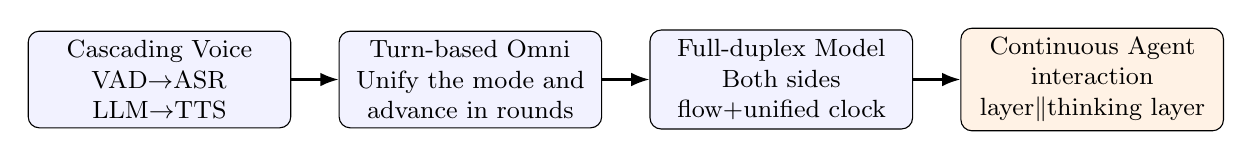
\begin{tikzpicture}[node distance=6mm,>=Latex,font=\small,
box/.style={draw,rounded corners,minimum height=10mm,text width=31mm,align=center,fill=blue!5},
arr/.style={->,thick}]
\node[box] (c1) {Cascading Voice\\VAD$\to$ASR\\LLM$\to$TTS};
\node[box,right=of c1] (c2) {Turn-based Omni\\Unify the mode and advance in rounds};
\node[box,right=of c2] (c3) {Full-duplex Model\\Both sides flow+unified clock};
\node[box,right=of c3,fill=orange!10] (c4) {Continuous Agent\\interaction layer$\parallel$thinking layer};
\draw[arr] (c1)--(c2);
\draw[arr] (c2)--(c3);
\draw[arr] (c3)--(c4);
\end{tikzpicture}
\caption{The key evolution of speech models is not to simply expand parameters, but to gradually remove text bottlenecks, turn barriers and single-time scale reasoning.}
\label{fig:evolution}
\end{figure}

\subsection{Official system profile of GPT-Live}

The online system described by \FOne OpenAI can be summarized into four planes. First, the \textbf{ media plane (media plane) } continuously sends and receives audio through WebRTC, and handles packet loss, jitter, clock drift and audio catch-up. Second, the \textbf{ interaction plane } runs the GPT-Live speech model and continuously decides when to speak, listen, stop, interrupt, call tools, or initiate delegation according to the audio clock. Third, \textbf{ cognitive plane } maintains a pre-created and populated frontier-model session with stable session affinity for undertaking complex reasoning. Fourth, \textbf{ control/state plane } maintains session state, transcript, context compaction, security control and instance handoff \cite{openai2026continuous,openai2026safety}.

Set up an asynchronous RPC\footnote{Remote Procedure Call between the media fast path and the application logic. } Boundaries are critical: neither database access, business logic, nor time-consuming tools can reversely block audio frames. The system therefore has two consistency levels: the audio path adopts a "time-limited priority" weak synchronization method, and the application state adopts retryable event semantics. Discrete semantic turns can still be derived on top of continuous audio, and both speculative transcript and authoritative transcript are maintained simultaneously. Therefore, "cancelling the turn detector" refers to canceling the turn gating that would block the audio path, rather than giving up semantic segmentation.

\begin{figure}[H]
\centering
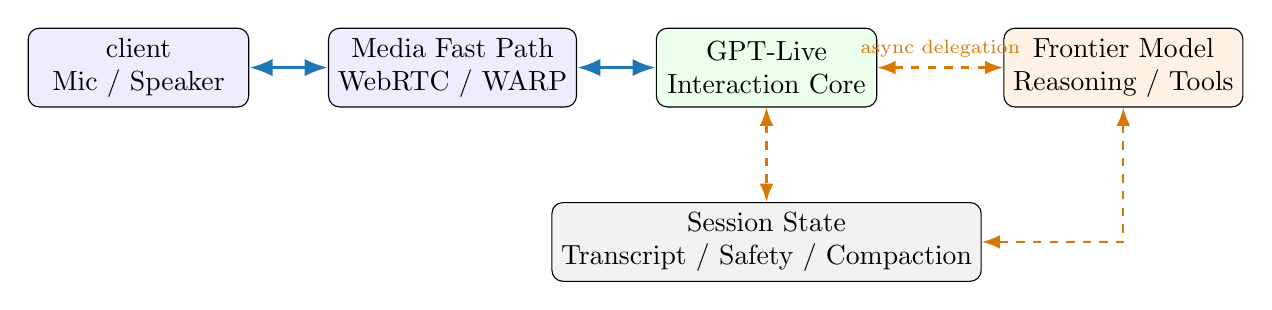
\begin{tikzpicture}[>=Latex,node distance=8mm and 10mm,
p/.style={draw,rounded corners,minimum width=28mm,minimum height=10mm,align=center},
fast/.style={->,very thick,official},slow/.style={->,thick,dashed,hypothesis}]
\node[p,fill=blue!7] (client) {client\\Mic / Speaker};
\node[p,fill=blue!7,right=of client] (media) {Media Fast Path\\WebRTC / WARP};
\node[p,fill=green!8,right=of media] (live) {GPT-Live\\Interaction Core};
\node[p,fill=orange!10,right=16mm of live] (think) {Frontier Model\\Reasoning / Tools};
\node[p,fill=gray!10,below=12mm of live] (state) {Session State\\Transcript / Safety / Compaction};
\draw[fast,<->] (client)--(media);
\draw[fast,<->] (media)--(live);
\draw[slow,<->] (live)--node[above,font=\scriptsize]{async delegation}(think);
\draw[slow,<->] (live)--(state);
\draw[slow,<->] (think)|-(state);
\end{tikzpicture}
\caption{Outlines of the GPT-Live system under evidence constraints. The solid blue line is the low-latency media closed loop, and the orange dashed line is the cognitive and state closed loop that allows higher latency. The logical layering in the figure comes from official facts; the internal implementation of the module remains undisclosed.}
\label{fig:official-architecture}
\end{figure}

\section{Formalizing Full-Duplex Continuous Inference}

The round-robin LLM only needs to ensure the causality on the token sequence; the full-duplex model must also ensure that the queuing and calculation time of each audio chunk meets $Q_t+C_t\leq\Delta$. Otherwise, even if the semantics are correct, lags will occur due to missing the playout deadline. Therefore, the state of continuous inference not only contains historical semantics, but also must synchronize user audio, assistant's own output, playback progress, tool events, and safety signals, and allow low-latency interaction paths and high-cost cognition paths to advance in parallel on different time scales.

\subsection{From token sequence to wall-clock constrained two-stream process}

The following formalization uses standard Transformer autoregressive modeling as a starting point \cite{vaswani2017attention}.

Ordinary autoregressive LLM modeling $p(y_n\mid x,y_{<n})$, input $x$ is fixed before decoding starts. Full-duplex speech is different: new user input continues to arrive while the assistant generates speech. Discretize the wall-clock into audio chunks of length $\Delta$, let $u_t$ represent the $t$ user audio chunk, $a_t$ represent the assistant output, $z_t$ represent the internal interaction action, and $m_t$ represent the persistent state, then the system needs to complete the following calculations before each playout deadline:
\begin{align}
m_t &= f_\theta(m_{t-1},u_t,\tilde a_{t-d:t-1},e_t),\\
(a_t,z_t) &\sim p_\theta(\cdot\mid m_t),\qquad
z_t\in\{\texttt{listen,speak,pause,stop,backchannel,delegate,tool}\}.
\end{align}
$\tilde a$ represents the system's own playback reference, or its own output after acoustic echo cancellation; $e_t$ represents tool results, network status, and safety signals. The most important constraint here is not the probability formula itself, but $C_t+Q_t\leq\Delta$: the sum of the calculation time $C_t$ of a single audio chunk and the queuing time $Q_t$ must be less than the playout deadline. Occasional timeouts will cause audio underrun, and continuous timeouts will appear as mechanical pauses.

Full-duplex contains at least four meanings: (1) The transport layer can be uplinked and downlinked at the same time; (2) The model continues to encode user input while speaking; (3) The policy layer can handle speech overlap, short responses and user interruptions; (4) The session layer remains interactive during the execution of background tasks. Merely having a two-way WebSocket connection cannot be called a full-duplex model; if the system freezes interaction when processing complex tasks, even if it has the first three layers of capabilities, it is not equivalent to the continuous agent emphasized by GPT-Live.

\subsection{State, Causality, and Echo}

The causal system can only use $u_{\le t}$, but in exchange for a more robust speech representation, has limited look-ahead $L$. The algorithm delay lower bound is approximately
\begin{equation}
T_{\mathrm{algo}}=T_{\mathrm{chunk}}+T_{\mathrm{lookahead}}+T_{\mathrm{codec}}+T_{\mathrm{decode}}.
\end{equation}
Reducing $\Delta$ will increase decision frequency, but increase token rate, kernel launch and scheduling pressure. Publicly available systems with a time grid of 80--160 ms represent a typical compromise: fast enough to respond to interruptions, yet able to accumulate discernible acoustic evidence within a grid \cite{defossez2024moshi,zhang2026duplexsla}.

The model must also differentiate between "the user is speaking" and "the speaker sound is being reacquired by the microphone." Traditional AEC\footnote{Acoustic Echo Cancellation, acoustic echo cancellation. } eliminates known playback references in the waveform domain; the model side can also explicitly receive assistant history, self-output token or echo flag. If only a single channel of mixed audio is used for training, the model may mistake its own voice for user instructions. SALMONN-omni lists echo cancellation as the full-duplex core scenario \cite{yu2025salmonnomni}, indicating that the evaluation must cover residual echo, double talk and different acoustic paths, and cannot only be tested on clean separate channels.

\subsection{Dual time scale control}

Control latencies for natural conversation are not the same as task reasoning latencies. The fast ring $\pi_f$ runs every $\Delta$ milliseconds and is responsible for maintaining contact and deciding whether to give up the floor; the slow ring $\pi_s$ may run for several seconds and is responsible for searching, planning, or calling tools:
\begin{equation}
\pi_f:(u_t,m_{t-1})\mapsto(a_t,z_t),\qquad
\pi_s:(q,M)\mapsto r,quad r\xrightarrow{\mathrm{event}}m_{t+k}.
\end{equation}
The difficulty with asynchronous delegation is how to re-inject the results into the current conversation: the results may be out of date, the task may be canceled by the user, or they may conflict with previous representations of the interaction layer. Therefore, the event should at least contain \texttt{task\_id}, context version, creation time, cancellation status and source information; after receiving the result, the interaction layer should also perform a correlation judgment instead of unconditional reading.

\section{Public Model Architectures: Components and Design Axes}

Although the public models in recent years have different implementation paths, they have gradually converged to the basic structure of "shared timeline, dual streams of users and assistants, and continuous status updates". What really affects the behavior of the system are three sets of tradeoffs: the uniformity of generation and high token rate of codec tokens, the semantic coupling capability and overlap interference of channel fusion, and the control accuracy and backbone burden of silence/control/action tokens. These design axes can explain the differences between Moshi, SyncLLM, LSLM, Neural-FSM and DuplexSLA, and also constitute a candidate mechanism space for understanding GPT-Live.

\subsection{Audio representation: continuous features, semantic tokens and codec tokens}

End-to-end voice LLM typically starts by downsampling the 16/24 kHz waveform to a low-frequency representation. SoundStream and EnCodec use a convolutional encoder, residual vector quantization (RVQ), and a generative decoder to compress the waveform into a multi-codebook discrete token\cite{zeghidour2021soundstream,defossez2022encodec}. If the frame rate is $f$, the number of codebooks is $K$, and the size of each dictionary is $V_k$, the original discrete code rate
\begin{equation}
R=f\sum_{k=1}^{K}\log_2V_k\quad\text{bit/s}.
\end{equation}
High-level codebooks tend to carry coarser semantics and prosody, with subsequent codebooks filling in the acoustic details. AudioLM further separates semantic tokens and acoustic tokens, uses lower-frequency semantics to ensure long-term consistency, and uses codec code to reconstruct the sound quality \cite{borsos2022audiolm}.

VITA-Audio uses multiple cross-modal token prediction to generate multiple audio tokens in one forward pass. The author reports that 3--5 times the inference speedup\cite{long2025vitaaudio} is obtained at the 7B scale, indicating that parallel acoustic decoding is an important direction to reduce time-to-first-audio.

The Codec-token route allows next-token prediction to cover both understanding and generation, but the token rate is very high. Assume 12.5 frames per second and 8 codebooks, that is, 100 audio tokens per second; if both streams exist at the same time, backbone throughput and KV cache\footnote{Key-Value cache, Transformer caches the Key and Value representation of historical tokens during incremental decoding to avoid repeated calculations. } growth will be significantly higher than text chat. Typical optimizations include delay pattern, hierarchical depth decoder, multi-token prediction, and semantic/acoustic layering. Moshi uses Temporal Transformer to model time, Depth Transformer to expand multiple codebooks in the same frame, and time-aligned text Inner Monologue to improve language quality \cite{defossez2024moshi}.

Another route does not inject the codec id into the LLM vocabulary. LSLM uses streaming SSL\footnote{Self-Supervised Learning, self-supervised learning; here it refers to learning continuous acoustic representations with unlabeled speech. } encoder provides continuous auditory features and token-based TTS to generate speech; SALMONN-omni emphasizes codec-free token space and dynamic thinking \cite{ma2025lslm,yu2025salmonnomni}. This approach reduces the acoustic entropy that the backbone needs to learn, but requires an external speech decoder to strike a balance between low latency and high fidelity. The two types of routes are essentially the difference in the division of labor on "how much acoustic details the backbone bears."

A recent review summarized related methods as "engineering synchronization" and "learning synchronization", which also confirmed that the model side and the system side need to evolve in parallel \cite{chen2025survey}.

\subsection{Representing Both Speakers in the Backbone}

\paragraph{Sequence flattening}
SyncLLM cuts real time into chunks and serializes user and assistant events with synchronization markers; OmniFlatten uses a unified flatten operation to cover modal alignment, half-duplex and full-duplex training \cite{veluri2024syncllm,zhang2024omniflatten}. The advantage is that it reuses standard decoder-only LLM and next-token loss. The disadvantage is that the sequence order may artificially break the symmetry of "the same moment" and the token rate will be inflated.

\paragraph{Parallel streams and multiple codebooks}
Moshi simultaneously models user and assistant audio streams, and dGSLM earlier used Twin Towers Transformer and cross-attention to generate speech, laughter and turn dynamics \cite{nguyen2022dgslm,defossez2024moshi} in two channels in parallel. Parallel representation is closest to the physical process, but batch, cache and loss mask all need to understand the two-dimensional time $\times$ channel structure.

\paragraph{Fusion and cross-attention}
LSLM compared early, middle and late fusion. A control experiment in 2026 further showed that channel fusion can establish stronger semantic connections, but it is also easier to interfere with the generated context when input overlap; using user stream as external memory and reading through cross-attention is more robust, but the question and answer ability is relatively weak \cite{ma2025lslm,lu2026routing}. Therefore, architecture evaluation cannot only look at static spoken QA, but must also examine semantic recovery after interruption.

\subsection{Representing Interaction Actions}

The simplest approach is to treat silence as an output: if the model generates a silence token at a certain time slot, it means that it has chosen to "continue listening". SyncLLM and Moshi can implicitly learn overlaps and pauses from the joint distribution of the user and assistant streams. Neural-FSM allows LLM to explicitly output the control token and drive a dual-state FSM\footnote{Finite-State Machine, a finite state machine. }, decide to start answering, continue waiting, or accept interruption; the paper reports that in simulation evaluation, its average response delay was more than three times lower than that of the half-duplex system, and more than half of the interactions could respond to \cite{wang2024neuralfsm} within 500 ms. Explicit control makes monitoring and auditing easier, but a state machine that is too coarse-grained can also limit the naturalness of interactions.

DuplexSLA combines decoding assistant audio with a rate-limited text action channel on a shared 160 ms timeline, allowing planning and tool invocation to occur in parallel with speech output\cite{zhang2026duplexsla}. This represents a more general speech--language--Action (Speech--Language--Action, SLA) modeling method: audio is responsible for low-bandwidth social feedback, and the action channel is responsible for high-precision structured control. GPT-Live officially only confirms that the system can continuously decide when to call tools or initiate asynchronous delegation; whether there are native action headers internally has not yet been disclosed.

\begin{table}[H]
\centering\scriptsize
\setlength{\tabcolsep}{3pt}
\caption{The core design axis of the full duplex public route. "GPT-Live" in the table only lists official public attributes, and the question mark indicates that it has not been disclosed.}
\begin{tabularx}{\textwidth}{lXXXXX}
\toprule
System & Input organization & Voice output & Interactive control & Deep reasoning & Main features \\
\midrule
Moshi & Dual parallel audio streams & RVQ codec & Implicit timing & Single trunk & Inner Monologue, about 200 ms Actual measurement \\
SyncLLM & time chunk flattening & HuBERT/voice unit & sync token & single trunk & real clock synchronization \\
Neural-FSM & serialized sensing event & modular motor & control token & within LLM & two-state FSM \\
LSLM & streaming SSL & token TTS & post-fusion prediction & single-backbone & early/middle/late fusion \\
OmniFlatten & flatten sequence & speech token & learning from data & single-backbone & three-stage post-training \\
SALMONN-omni & Continuous speech features & Independent generation module & dynamic thinking & Single backbone & codec-free token space \\
DuplexOmni & streaming audio/video & streaming voice & interaction layer & asynchronous plug-in & interaction -- thinking decoupling \\
DuplexSLA & Dual-stream three-channel & Discrete audio & action channel & Same as trunk action & Shared 160 ms clock \\
GPT-Live & Continuous audio & Continuous voice & Continuous decision-making & Asynchronous delegation & tokenizer/fusion Undisclosed \\
\bottomrule
\end{tabularx}
\end{table}

\subsection{The essential difference from the end-to-end Omni Model}

The two are not mutually exclusive concepts. Omni emphasizes \emph{ modal unity }: the same model can understand and generate text, images or audio; full-duplex emphasizes \emph{ time and control unity }: new inputs can continue to arrive during the generation process, and the model can sense wall-clock, and maintain the correct causal state when speech overlaps. A model can be Omni but still interact on a turn-by-turn basis, or it can be full-duplex capable but only handle audio.

GPT-Live further introduces \emph{ capability decoupling }: the low-latency interactive core does not have to bear all complex reasoning. Rather than having the very large omni model complete an expensive inference every 80--160 ms, this solution allocates "frame-level decisions that cannot be missed" and "tasks that can wait but require smartness" to different computing paths. This is both product experience design and the core of serving feasibility.

\section{Training data and post-training}

\subsection{Why Is Ordinary Voice Q\&A Data Insufficient?}

Turn-based SFT\footnote{Supervised Fine-Tuning, supervised fine-tuning. } samples usually only have "complete user audio $\to$ complete assistant answer", with almost no overlap, hesitation, short feedback, talk grabbing, cancellation and self-correction. The model is ASR, SQA\footnote{Spoken Question Answering, spoken question answering. } and TTS are both very strong, and they will only wait for the end of the clear sentence. Full-duplex training samples should be binaural, shared timeline event sequences
\begin{equation}
D=\{(u_{1:T},a_{1:T},c_{1:T},s_{1:T},q,r)\},
\end{equation}
Among them, $c_t$ is the interaction action, $s_t$ is the speaker/overlapping state, and $q,r$ is the optional delegation request and return. Data must not only answer "what to say" but also monitor "when to speak, when to remain silent, and when to stop."

Real binaural data are scarce and privacy sensitive. SyncLLM trained the clock synchronization capability \cite{veluri2024syncllm} with 212k hours of synthetic speech dialogue and 2k hours of real dialogue; DuplexChat-Pipe performed language filtering, download cleaning, diarization, dual-person segment extraction, speech separation and restoration from public podcasts, and the author reported output of 282,634 hours of English and 132,723 hours of Japanese data \cite{nakata2026duplexchat}. These scales mean that data engineering has become a major constraint on model capabilities, but automatic separation introduces crosstalk, mis-speakers, false overlaps and recovery artifacts, and quality tags must be preserved rather than just reported in hours.

\subsection{Suggested Progressive Training Recipes}

Progressive training is commonly used in public work. OmniFlatten sequentially performs modal alignment, half-duplex dialogue learning, and full-duplex dialogue learning \cite{zhang2024omniflatten}; Freeze-Omni freezes the text backbone, first accesses the voice input and output modal, and then performs duplex multi-task training \cite{wang2024freezeomni}. A reproducible six-stage training program is as follows:

\begin{enumerate}
\item \textbf{Representation pretraining: } optimizes reconstruction quality, semantic fidelity, streaming causality and low frame rate to establish a stable representation under clean/noisy/echo conditions.
\item \textbf{Speech--text alignment: } mixes ASR, TTS, speech continuation, and spoken QA to align speech capabilities with the text backbone; replay text capabilities to avoid catastrophic forgetting.
\item \textbf{Half-duplex dialogue: } Learn command following, roles, voice style and long context to ensure "what to say" converges first.
\item \textbf{Synthetic duplex conversion: } expands text conversations into timestamped binaural audio, randomly sampling pauses, backchannels, overlaps, barge-in and network delays.
\item \textbf{Real duplex adaptation: } uses real two-channel dialogue to calibrate time distribution, prosody and cultural differences, reducing template bias in synthetic data.
\item \textbf{Preference/RL\footnote{Reinforcement Learning, reinforcement learning. }: } optimizes interruption accuracy, error grabbing, task completion, conversation redundancy and recovery capabilities; introduces safety interrupt and delegate policy.
\end{enumerate}

The loss can be written as
\begin{equation}
\mathcal L=\lambda_a\mathcal L_{audio}+\lambda_t\mathcal L_{text}+\lambda_c\mathcal L_{control}
+\lambda_{asr}\mathcal L_{align}+\lambda_s\mathcal L_{safety}+\lambda_d\mathcal L_{delegate}.
\end{equation}
The magnitudes of tokens corresponding to different losses vary greatly. The density of audio tokens is much higher than that of control tokens; if simply averaged by token, the model will prioritize optimizing acoustic details and ignore rare but critical correct interruptions. Therefore, control/action events should be reweighted, and precision/recall should be reported by scenario instead of just looking at the total loss.

\subsection{Quantifiable quality control of data pipelines}

It is recommended that the following quality fields be retained for each audio segment: Speaker Purity, Overlap Ratio, Signal-to-Noise Ratio, Residual Echo, Speaker Separation Confidence, Speech Separation Artifact Score, Language and Accent, Turn Switch Interval, Short Answer Label, Privacy and Security Label, and Licensed Source. Key thresholds include: (1) Crosstalk leakage is determined when binaural cross-correlation is too high; (2) Sample weights are reduced when ASR transcription is inconsistent with the speaker's timeline; (3) Extreme negative intervals and long overlaps are bucketed separately; (4) Between the training set and the evaluation set, the same podcast, the same speaker, and near-duplicate audio are deduplicated.

For synthetic data, \emph{ two-way calibration } is required: first, the target distribution of the round switching interval, overlap duration and short response frequency is given by the real data, and the synthesizer then samples according to these distributions; after the training is completed, it is also necessary to check whether the model output deviates from the true distribution. Simply pursuing lower response latency will induce the model to frequently grab calls, so the false interruption rate must also be used as a protection indicator.

\section{Stateful Serving: Delivering Audio Frames on Time}

The upper limit of the capacity of real-time voice serving is not how many requests are completed per unit time, but how many concurrent sessions can continue to generate audio frames before their respective playout deadlines; the average RTF\footnote{Real-Time Factor, real-time factor; usually refers to the ratio of the time required to process a piece of audio to the length of the audio piece. } less than 1 may still cover up consecutive deadline misses caused by burst prefill. Long sessions will also cause the KV cache to continue to grow with audio tokens, so context compaction must be moved out of the live path, and smooth handoff must be completed through background prefill, parallel running, and safe cut-over of the replacement instance.

\subsection{From Request Capacity to Session-Frame Capacity}

Text serving can use single request latency instead of throughput; real-time voice cannot make the session wait for long prefill.

\FOne OpenAI clearly measures capacity by "how many concurrent sessions can continue to process frames on time" instead of GPU request throughput\cite{openai2026continuous}.

Assuming that the active session set is $S$ and the $i$ session frame budget is $\Delta_i$, the more reasonable SLO\footnote{Service-Level Objective is the service level objective. } Yes
\begin{align}
\mathrm{DMR} &= \frac{\sum_{i,t}\mathbf 1[Q_{i,t}+C_{i,t}>\Delta_i]}{\sum_iT_i},\\
\mathrm{GoodSessions} &= \sum_i\mathbf 1[\mathrm{DMR}_i<\epsilon\land P_{99}(J_i)<J_{max}],
\end{align}
Here we measure the deadline-miss ratio (DMR) \footnote{Deadline-Miss Ratio respectively, which is the proportion of frames that failed to complete before the deadline. } and the number of concurrent sessions that meet the jitter threshold. Even if the average real-time factor (RTF) is lower than 1, the interactive experience is not guaranteed because sudden context prefill may still cause continuous frame misses.

The scheduler should use deadline-aware continuous batching: sort audio frames according to the latest playout deadline; limit the size of each batch of context prefill; reserve computing power for audio decode; put background context compaction, transliteration revision, and delegation model prefill into a low-priority queue. When the load is too high, you should successively reduce non-critical telemetry, reduce the intensity of acoustic refinement, delay background tasks, and finally consider sacrificing the quality of the interactive core.

\subsection{KV cache and continuous context}

Transformer-XL's segment recurrence is an earlier cross-segment memory solution \cite{dai2019transformerxl}, but real-time voice also requires that the state and playback time are strictly consistent.

The Transformer KV cache grows over time at every layer. Its GPU-memory footprint is approximately
\begin{equation}
M_{KV}\approx 2LNH_{kv}d_hb,
\end{equation}
Among them, $L$ is the number of layers, $N$ is the cumulative token, $H_{kv}$ is the number of KV heads, $d_h$ is the head dimension, and $b$ is the bytes per element. The combination of high audio token rate and long sessions makes the cache become the session capacity bottleneck. PagedAttention reduces dynamic cache fragmentation and duplication through paging, and FlashAttention reduces attention to HBM access \cite{kwon2023pagedattention,dao2022flashattention} through IO-aware tiling; but they do not automatically resolve infinite contexts.

Hierarchical memory can be used: (1) retain the original dual-stream token for the most recent $W$ seconds to ensure interruption processing and reference resolution; (2) compress earlier speech into final transcription and event summary; (3) retain structured provenance for tool results; (4) write user preferences into independent long-term states. Compression is not a lossless operation, it changes the token prefix and invalidates the old KV cache. \FOne OpenAI moves the context compaction out of the live path, completes the prefill of the replacement instance in the background, and then switches to \cite{openai2026continuous}, thereby preventing the main instance from stalling due to long context prefill.

\subsection{Seamless instance switching}

Stateful sessions cannot be arbitrarily load balanced like normal HTTP requests. The officially described switching process is: start and warm up replacement; prefill with compressed context; run new and old instances in parallel; cut over at safety boundaries. This process simultaneously addresses context compression, instance maintenance, and failure recovery.

\begin{figure}[H]
\centering
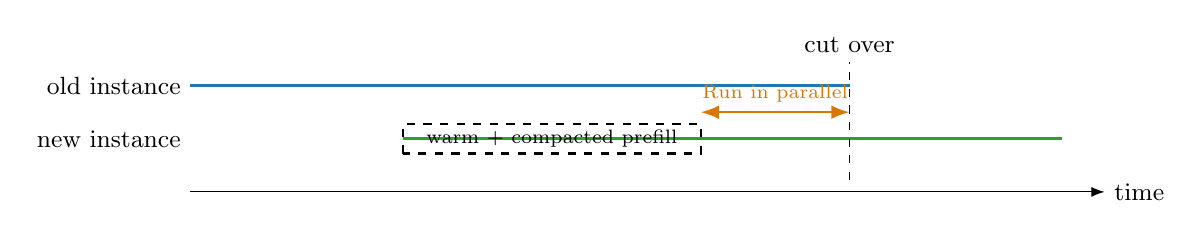
\begin{tikzpicture}[>=Latex,x=1.35cm,y=0.75cm,font=\small]
\draw[->] (0,0)--(8.6,0) node[right]{time};
\node[left] at (0,1.8){old instance}; \node[left] at (0,0.9){new instance};
\draw[very thick,official] (0,1.8)--(6.2,1.8);
\draw[very thick,public] (2.0,0.9)--(8.2,0.9);
\draw[thick,dashed] (2.0,0.65) rectangle (4.8,1.15);
\node[font=\scriptsize] at (3.4,0.9){warm + compacted prefill};
\draw[<->,hypothesis,thick] (4.8,1.35)--(6.2,1.35) node[midway,above,font=\scriptsize]{Run in parallel};
\draw[dashed] (6.2,0.2)--(6.2,2.2) node[above]{cut over};
\end{tikzpicture}
\caption{Stateful reasoning instance switching. Switching points should be at recoverable acoustic boundaries, and duplicate/missing frames should be deduplicated.}
\end{figure}

There are three types of race conditions that need to be dealt with in the project: the tool results arrive exactly during the instance switch; the final transcriber revise the old text; and the user interrupts at the flow boundary. It is recommended to attach a monotonically increasing sequence number and context epoch to all events; the new instance only accepts state changes matching the epoch, and deduplicates the media frame according to the playout timestamp.

\subsection{Asynchronously delegated serving design}

\FOne In order to reduce the first response delay of complex tasks, the system will pre-create and populate the frontier-model session, maintain stable session affinity, and utilize prompt caching\cite{openai2026continuous}. The time taken for delegation can be broken down into
\begin{equation}
T_{delegate}=T_{route}+T_{queue}+T_{prefill\_delta}+T_{reason}+T_{tool}+T_{return}.
\end{equation}
Pre-population can only reduce $T_{prefill\_delta}$; inference strength, the size of the tool pattern definition, and the number of serial tool call rounds still determine long-tail latency. Therefore, the interaction layer needs to adopt progressive feedback: first use a short response to inform the user that the task is being processed, and then choose the appropriate time to insert after the result arrives; if the user has changed the topic, cancel the background task or reduce its priority.

Speculative decoding can first generate a draft from a small model and then hand it over to a large model for parallel verification, reducing the serial decoding step\cite{leviathan2023speculative} without changing the target distribution; however, it is more suitable for the cognition path and cannot replace the scheduling with hard deadline constraints in the interaction path.

Security policies must also be consistent across layers. The GPT-Live system card claims that the security system continuously checks input and output along with the conversation and can steer, interrupt, play a security response or end the session \cite{openai2026safety}. This means that security controls cannot just sit at the end of the delegated model, otherwise the real-time layer may have generated inappropriate speech before the long inference returns.

\section{Real-time networking: WebRTC, WARP and playout clock}

\subsection{Why not "just switch to WebSocket"}

WebRTC converts media, NAT\footnote{Network Address Translation, network address translation; NAT traversal refers to establishing an end-to-end connection across address translation devices. } penetration, congestion control, security and data channels are combined into a browser real-time communication stack. In standard WebRTC, media usually passes through the SRTP\footnote{Secure Real-time Transport Protocol. }, non-media data channel uses SCTP over DTLS over ICE/UDP \footnote{SCTP: Stream Control Transmission Protocol, flow control transmission protocol; DTLS: Datagram Transport Layer Security, datagram transport layer security protocol; ICE: Interactive Connectivity Establishment, interactive connection establishment; UDP: User Datagram Protocol, user datagram protocol. }\cite{alvestrand2021webrtc,jesup2021datachannels}. Audio frames have different reliability requirements than tool events: old audio packets that arrive late are usually not worth retransmitting, while tool results and status changes need to be reliable and orderly. Putting both into a reliable byte stream creates head-of-line blocking.

The end-to-end perceived delay can be written as
\begin{equation}
T_{e2e}=T_{capture}+T_{uplink}+T_{jitter,in}+T_{model}+T_{downlink}+T_{jitter,out}+T_{playout}.
\end{equation}
If the 20 ms saved on the model side is offset by the 300 ms connection setup or jitter buffer, the user will not perceive this part of the optimization. On the contrary, if the jitter buffer is too small, it will increase the number of missing frames in a weak network environment. The system should be based on recent packet loss, RTT\footnote{Round-Trip Time, and round-trip delay, which is the time required for data to travel from the sender to the receiver and back again. } and clock drift dynamically adjust the playout policy instead of setting the same fixed parameters for the global network.

SimulTron's end-side synchronous speech-to-speech translation is also jointly designed with the causal encoder, adjustable fixed delay and streaming vocoder \cite{agranovich2024simultron}, indicating that both the model algorithm and the audio playback path must be taken into account when evaluating delay.

\subsection{Optimization of connection establishment from 6 RTT to 1 RTT}

\FOne OpenAI collectively refers to related WebRTC optimizations as WARP, saying that the establishment of media and data channels is reduced from 6 round trips to 1, combined with SPED\footnote{STUN Protocol for Embedding DTLS; where STUN is Session Traversal Utilities for NAT. This draft embeds DTLS handshake data and acknowledgment into STUN Binding messages. }, DTLS 1.3, SNAP\footnote{SCTP Negotiation Acceleration Protocol, put SCTP initialization parameters into SDP offer/answer to reduce serial round-trips for data channel establishment. } and pre-negotiated data channel\cite{openai2026continuous}. DTLS 1.3 itself uses the shorter handshake mode \cite{rescorla2022dtls13}; SPED embeds DTLS handshake data/ack into STUN Binding Request/Response; SNAP embeds SCTP initialization parameters into SDP\footnote{Session Description Protocol. } offer/answer, thereby reducing the serial round trip of the data channel \cite{hancke2026sped,hancke2026snap}. The latter two are still Internet-Draft as of this writing and cannot be considered stable RFC\footnote{Request for Comments, a series of standards, specifications, or informational documents in the field of Internet engineering and protocols. }.

Instant Connect goes one step further and pre-negotiates SDP, allowing the client to start session \cite{openai2026continuous} with a single UDP packet. This requires the server to allocate or restore sufficient connection status in advance, and also introduces anti-replay, resource abuse, and reservation expiration issues. Low RTT is not a free lunch: the more aggressive the state warm-up, the higher the cost due to air connections and attack traffic.

\subsection{Packet Loss, Clock Drift, and Audio Catch-Up}

The client sampling clock, server generation clock and speaker playout clock are not completely consistent. If the generation is slightly slower, the buffer will gradually be exhausted; if the generation is slightly faster, the buffer accumulation will cause the interaction to become later and later. The official article mentions audio time stretching/catch-up\cite{openai2026continuous}: Adjust the playout rate within a small range or selectively discard low-value segments to bring the delay back to the target range. Implementations should limit the stretching ratio and operate at the voice activity boundary to avoid pitch and prosody distortion.

The weak network test at least covers independent random packet loss and burst loss, uplink/downlink asymmetry, RTT burst, NAT rebinding, Wi-Fi/cellular switching, client background recovery and audio device switching. The evaluation is not only the ASR after packet loss WER\footnote{Word Error Rate, the word error rate is usually calculated based on the number of substitution, deletion and insertion errors relative to the reference word count. }, also includes whether the assistant repeats, grabs the call, forgets the user's mid-course correction, and whether the tool events are consistent with the audio status.

\section{Evaluation: From Model Scores to Continuous Interaction Quality}

\subsection{Four-tier evaluation framework}

Full-Duplex-Bench splits the core interaction behaviors into pause processing, short responses, turn switching and interruption management \cite{lin2025fullduplexbench}; v2 further adds multi-round stage goals, fast and slow speaking rhythms, error correction, entity tracking and security tasks \cite{lin2026fullduplexbenchv2}. Combined with the online system requirements, it is recommended to conduct evaluation from the following four levels:

\begin{enumerate}
\item \textbf{ Acoustics/Semantics: }ASR WER, spoken QA accuracy, speaker similarity, MOS\footnote{Mean Opinion Score, average subjective opinion score, usually evaluated by the listener for naturalness or quality of speech; UTMOS is automatically predicted MOS Neural network evaluator. }/UTMOS, mood and prosody following, noise/accent robustness.
\item \textbf{ Interaction behavior: } initial response delay, pause/overlap distribution, accuracy and recall rate of short responses, stop delay after user interrupts, false interruption rate, and semantic consistency after recovery.
\item \textbf{ agent tasks: } tool calling accuracy rate, parameter exact matching rate, delegation trigger accuracy and recall rate, task completion rate, cancellation instruction compliance rate, result timeliness and source information accuracy rate.
\item \textbf{ System service quality: }connection RTT, first audio delay, audio frame deadline-miss ratio, jitter, playout buffer underrun, handoff gap, single session GPU memory, number of sessions each GPU can stably carry, and cost per minute.
\end{enumerate}

There are cultural differences in human turn-taking itself\cite{stivers2009turntaking}, therefore the single "faster, better" cannot be regarded as a natural goal. The full distribution of transition gaps should be reported, and the reviewer should be asked to simultaneously rate response relevance, abruptness, verbosity, and respect for interruptions.

\subsection{Key Metric Definitions}

Assume that the user starts interrupting at time $t_b$ and the assistant stops audible speech at time $t_s$, then the stop delay is $t_s-t_b$; only when the user input does constitute a valid semantic interruption, it will be recorded as a real example. defined by this
\begin{equation}
P_{int}=\frac{N_{correct\ stop}}{N_{all\ stop}},\qquad
R_{int}=\frac{N_{correct\ stop}}{N_{valid\ barge\mbox{-}in}}.
\end{equation}
Optimizing only $R_{int}$ may cause the model to stop speaking due to coughing or short responses; optimizing only $P_{int}$ may cause the model to appear to be "rushing to talk" all the time. Therefore, $F_1$, cessation latency quantile, and recovery success rate should be reported simultaneously.

Delegation should be evaluated counterfactual: compare no delegation, synchronous delegation, and asynchronous delegation for the same task. Metrics include interaction stall, final accuracy, first useful feedback, tool round trips, and wasted computing power after user cancellation. The value of an asynchronous approach is not to make the final answer necessarily faster, but to keep the conversation available during slow tasks.

\subsection{Experiment Matrix and Attribution Principles}

To avoid confounding factors, it is recommended to fix the backbone, training token, duplex/real data ratio, codec, hardware and network trace, and only change one design axis. FIFO\footnote{First In, First Out in the table. } and EDF\footnote{Earliest Deadline First, the earliest deadline takes precedence. } is a two-type scheduling baseline, and the core ablation is as follows:

\begin{table}[H]
\centering\small
\caption{Proposed attributable ablation experiments.}
\begin{tabularx}{\textwidth}{p{3.0cm}p{4.0cm}X}
\toprule
Design axis & Control group & Main indicators and expected risks \\
\midrule
User flow routing & Channel fusion / cross-attention / gated mixing & SQA, post-overlap semantic interference, stop delay \\
Time granularity & 40/80/160/320 ms & DMR, interrupt delay, token throughput, voice naturalness \\
Action expression & Only silence token / FSM control token / action channel & Control accuracy, precise matching of tool parameters, backbone burden \\
Training plan & Direct full-duplex / three-stage / six-stage & Convergence, text ability forgetting, real interaction scoring \\
Thoughts on interaction -- & Single model / synchronous delegation / asynchronous delegation & Interaction pause, task accuracy, cost, cancellation waste \\
Context management & sliding window / summary / background handoff & long-session consistency, handoff gap, KV-cache GPU memory \\
Scheduling strategy & FIFO / continuous batching / EDF + computing power reservation & Stable number of sessions per GPU, DMR, P99 jitter \\
Network & Standard WebRTC / 1-RTT optimization / pre-connected & connect latency, security and air connection cost \\
\bottomrule
\end{tabularx}
\end{table}

Each result reports at least the mean, and P50/P95/P99\footnote{ represent the 50th, 95th, and 99th percentiles respectively; P99 is often used to observe the long-tail delay of the system. }, confidence interval and sample size by scenario. The randomness of the speech model and network traces will amplify the variance; if only one demo or average latency is reported, architectural conclusions cannot be supported.

\section{GPT-Live architecture reconstruction under evidence constraints}

Public evidence can confirm that GPT-Live continuously listens when making sounds, makes interaction decisions based on fine-grained clocks, and asynchronously delegates complex tasks to the frontier model; but these facts are not enough to deduce its specific tokenizer, fusion location, or action head. The minimal reconstruction that satisfies these constraints is a hybrid architecture: the media fast path carries continuous audio, the stateful interaction core maintains the two-stream causal state, the action channel triggers tools and delegation, the asynchronous cognition plane handles slow inference, and the authoritative state handles transcription, security, and context compaction.

\subsection{Which parts can be determined}

Based on official materials, the following system properties can be determined: \FOne (1) The speech model continues to listen when speaking, and does not use the traditional turn detector as a driving condition for audio processing; (2) The model decides multiple times per second when to speak, listen, pause, accept interruptions, call tools, or initiate delegation; (3) Complex tasks can be delegated asynchronously while maintaining uninterrupted interaction; (4) The media fast path and application logic are controlled by asynchronous RPC. Isolation; (5) Session inference has persistent state and supports background pre-population and instance switching; (6) Context compression does not block the real-time path; (7) WebRTC/WARP, packet loss processing and clock drift correction jointly determine the end-to-end experience; (8) System capacity is measured by whether the session audio frame can be completed on time \cite{openai2026gptlive,openai2026continuous}.

Together, these properties rule out two oversimplified explanations. First, GPT-Live is unlikely to be just "faster ASR, LLM, and TTS" because such pipelines rely on discrete rounds and cannot naturally handle new inputs arriving during the system's voicing. Second, it should not be understood as "one very large model taking on all tasks", because the official statement clearly states that the system will asynchronously hand over complex tasks to the cutting-edge model for processing.

\subsection{The most credible but unconfirmed internal mechanism}

The \Hyp interaction core is likely to have an internal state equivalent to a dual-stream time grid: each chunk encodes new user audio and recent self-output, updates the causal state, and then generates the assistant acoustic unit and interaction action. The representation may be like Moshi's parallel stream, SyncLLM's synchronized sequence, LSLM's continuous encoder plus fusion, or it may be an undisclosed new structure; the public information is not enough to choose one of the two.

\Hyp In order to understand the user while it is speaking, the system must obtain at least one self-speech reference: waveform-level post-AEC audio, model generation token, playback timestamp, or a combination thereof. Otherwise residual echo will be confused with real user input. The official mentions audio clock and playback catching up, but does not disclose how the echo reference enters the model.

\Hyp "Interaction model delegation frontier model" can be realized through structured events: the interaction model outputs the delegate intent and the compressed query, and the application server sends the final confirmed context and tool schema to the preheated session; the return result is written into the event stream, and then the interaction model chooses the appropriate time to convert it into natural spoken language. This process neither requires the speech model to expose its internal thinking, nor does it require the two models to share the KV cache.

\begin{figure}[H]
\centering
\resizebox{\textwidth}{!}{%
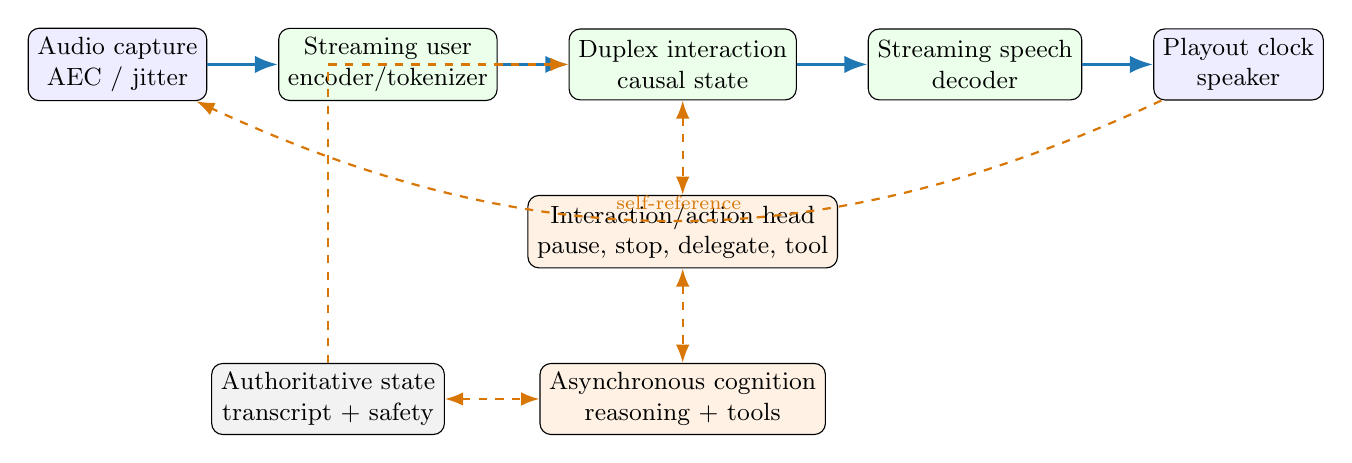
\begin{tikzpicture}[>=Latex,node distance=7mm and 9mm,font=\small,
box/.style={draw,rounded corners,align=center,minimum height=9mm},
f/.style={->,very thick,official},e/.style={->,thick,dashed,hypothesis}]
\node[box,fill=blue!7] (mic) {Audio capture\\AEC / jitter};
\node[box,fill=green!8,right=of mic] (enc) {Streaming user\\encoder/tokenizer};
\node[box,fill=green!8,right=of enc] (core) {Duplex interaction\\causal state};
\node[box,fill=green!8,right=of core] (dec) {Streaming speech\\decoder};
\node[box,fill=blue!7,right=of dec] (play) {Playout clock\\speaker};
\node[box,fill=orange!10,below=12mm of core] (action) {Interaction/action head\\pause, stop, delegate, tool};
\node[box,fill=orange!10,below=12mm of action] (frontier) {Asynchronous cognition\\reasoning + tools};
\node[box,fill=gray!10,left=12mm of frontier] (state) {Authoritative state\\transcript + safety};
\draw[f] (mic)--(enc); \draw[f] (enc)--(core); \draw[f] (core)--(dec); \draw[f] (dec)--(play);
\draw[e] (play) to[bend left=25] node[above,font=\scriptsize]{self-reference}(mic);
\draw[e,<->] (core)--(action); \draw[e,<->] (action)--(frontier); \draw[e,<->] (state)--(frontier); \draw[e] (state)|-(core);
\end{tikzpicture}%
}
\caption{Minimal architectural reconstruction that enables GPT-Live's public behavior. The green internal structure of speech and the orange action head are hypothetical; what is officially confirmed are continuous interaction, asynchronous delegation and system boundaries.}
\label{fig:reconstruction}
\end{figure}

\subsection{"Hybrid architecture" is more accurate than "pure end-to-end"}

On the perceptual -- vocalization path, end-to-end learning can preserve prosody, overlap, and non-verbal signals; on the complex task path, modular delegation allows the use of stronger reasoning models, tool permissions, and independent scaling; at the transport/state layer, deterministic protocols and explicit state machines are still irreplaceable. Therefore, GPT-Live is more like "an end-to-end interactive model embedded in a modular real-time system" rather than a single model annexation of all components.

This split also brings security and cost advantages: small and fast interactive models can be run frequently, and expensive models are only started when necessary; tool permissions are concentrated on the auditable cognitive plane; security controls can act on both real-time output and background results. The price is that cross-layer consistency, expired result processing, delegation strategies and session state recovery will be more complex.

\section{A reproducible open source implementation}

\subsection{Minimum Viable Architecture}

It is recommended to implement the research prototype as three independent services:

\begin{enumerate}
\item \textbf{Realtime gateway: }WebRTC ingress/egress, Opus, AEC/jitter buffer, playback timestamp, connection and weak network telemetry. Media packets go into bounded ring buffers, and application events go into reliable data channels.
\item \textbf{Duplex inference worker: } includes causal audio encoder, text LLM backbone, user-stream adapter, assistant audio decoder and action head. Workers maintain a fixed session affinity and perform an inference tick every 80 or 160 ms.
\item \textbf{Agent and state service: } are responsible for final transcription, conversation event log, tool runtime, reasoning model, context compaction, security policy and instance handoff coordination.
\end{enumerate}

The prototype can start from the voice backbone of the Moshi open source stack \cite{defossez2024moshi} and add independent action vocabulary and asynchronous tool bus; it can also adopt the Freeze-Omni/LSLM route, freeze the text LLM, and connect to the streaming encoder and lightweight audio decoder to reduce training costs \cite{wang2024freezeomni,ma2025lslm}. In the first stage, it is not appropriate to pursue video, long context, and multi-tool capabilities at the same time. The audio frame deadline and interruption behavior under real double-talk conditions should be verified first.

\subsection{Frame level scheduling pseudocode}

\begin{algorithm}[H]
\caption{Deadline-aware duplex session loop}
\begin{algorithmic}[1]
\ForAll{active session $s$ in earliest-deadline order}
  \State $u_t\gets$ readAudioChunk$(s,\Delta)$
  \State $e_t\gets$ drainReadyEvents$(s,\mathrm{contextEpoch})$
  \State $(a_t,z_t,m_t)\gets$ duplexStep$(u_t,e_t,m_{t-1})$
  \If{$z_t$ requests delegation and no equivalent task is active}
    \State enqueueAsync$(taskId,\mathrm{contextEpoch},\mathrm{query})$
  \EndIf
  \If{safety permits $a_t$ and playout deadline remains}
    \State sendAudio$(s,a_t,\mathrm{timestamp})$
  \Else
    \State applyGracefulDegradation$(s)$
  \EndIf
\EndFor
\State run background prefill, compaction, and telemetry with residual budget
\end{algorithmic}
\end{algorithm}

The scheduling loop needs to avoid three hidden blocking points: serial execution of the tokenizer or audio codec on the CPU; waiting for the final ASR transcript before updating the status; and incorrectly synchronously waiting for tool tasks in the media coroutine. All time-consuming operations should return results through events, and the media loop only consumes ready events.

\subsection{Phased experimental plan}

\paragraph{Phase A: Offline learnability}
Fixed 7B--9B text backbone and audio representation, and compared channel fusion, cross-attention and gated fusion under the condition that the number of training tokens is the same. The training set contains both half-duplex dialogue, synthetic overlap speech, and small-scale real binaural data. The acceptance criteria include: the degradation of spoke QA relative to the half-duplex baseline does not exceed the preset threshold; the recall of effective barge-in is improved and the false interruption rate does not deteriorate; self-trigger does not occur when echo exists.

\paragraph{Phase B: Single-machine real-time performance}
Gradually increase concurrent sessions on the fixed GPU, and record $Q/C$, DMR, P95/P99 jitter, KV cache memory and audio buffer underrun of each tick. Compare strategies such as FIFO, continuous batching, earliest deadline first (EDF), and reserved 20\% computing power. Acceptance is not based on the highest token throughput, but on the number of sessions that each GPU can stably carry.

\paragraph{Phase C: Asynchronous cognition}
Access a text reasoning model and three types of tools: low-latency query, long-latency search, and multi-round parameter completion. Compare the three modes of non-delegation, blocking delegation and asynchronous delegation, and check the tool result accuracy rate, interaction pauses, result expiration rate, computing power waste after task cancellation, and the user's subjective waiting experience.

\paragraph{Phase D: Long sessions and failures}
Run long sessions of 30, 60 and 120 minutes, actively injecting instance restart, network handoff, context compaction, transcript revision and tool-result race. The acceptance criteria include: there will be no duplication or deletion of speech during instance handoff; the context epoch will remain consistent; key user facts will be retained; and the GPU memory will not grow infinitely with the session duration.

\subsection{Resource and latency budget example}

When 160 ms is used as an inference tick, the following reference budget can be used: uplink and jitter buffer 40 ms, streaming encoder 15 ms, interaction backbone queuing and compute 45 ms, audio head and codec 20 ms, downlink, jitter buffer and playout 40 ms. This is not a public parameter of GPT-Live, just a starting point for engineering. Budgets must be verified using P95/P99 instead of average, and retested across geographies, low-end clients, and 5\% burst loss.

The cost model should be broken down by session minutes into interaction GPU, cognition GPU, audio bandwidth, tool calls, and idle reservation. If the delegation rate is $p_d$, the average reasoning time is $T_r$, and the interactive core cost per minute is $C_f$, the rough cost is
\begin{equation}
C_{min}=C_f+p_dT_rC_s+C_{net}+C_{tool}+C_{idle}.
\end{equation}
Reducing $p_d$ can save costs, but may also hurt task accuracy; therefore, it should be tuned together with delegation accuracy, recall, and final task success rate.

\section{Limitations, Open Questions, and Conclusions}

\subsection{Key details still unknown}

This report cannot determine GPT-Live's parameter count, training data, codec, audio-token rate, fusion-layer placement, use of joint action tokens, echo-reference injection, inference parallelism, or deployment scale because OpenAI has not publicly disclosed these details. Figure~\ref{fig:reconstruction} is a minimal implementation consistent with the publicly described behavior, not a leak or a reverse-engineering result.

It is also difficult to fairly compare existing papers. Moshi's "~200 ms", Neural-FSM's "response within 500 ms", GPT-4o's "average 320 ms" using different tasks, networks, hardware and latency starting points. This article reserves these numbers to illustrate their respective design goals and does not rank them into a unified ranking.

\subsection{Research Frontiers}

The most noteworthy directions in the future include: (1) adaptively selecting user-stream routing between strong semantic integration and resistance to overlap interference; (2) placing speech, language and action on a unified clock while avoiding high-frequency acoustic tokens from overwhelming sparse actions; (3) using real binaural data to train models that can adapt to different cultural turn-taking habits; (4) establishing factual fidelity and reversible audit mechanisms for long session compaction; (5) jointly optimizing inference tick, GPU scheduling, network jitter and playout clock; (6) Establish an asynchronous delegation benchmark covering stale result, task cancellation and provenance tracking.

\subsection{Conclusion}

The core of GPT-Live is not a mysterious acoustic module, but the reconstruction of a voice agent into a continuously running real-time system. Compared with the round-based full-modal model, it allows new inputs to continuously enter the model state during generation and synchronizes the interaction strategy with the real time; compared with the early single-model full-duplex solution, it further puts complex cognitive tasks into asynchronous paths for processing, and through stateful reasoning services, background context compression and instance switching, and low round-trip latency WebRTC, the model capabilities are transformed into a stable product experience.

Therefore, reproducing GPT-Live should not start with "training a larger speech LLM" starts, four closed loops should be established at the same time: \textbf{ represents the closed loop } to ensure that speaking and listening can be done in parallel, \textbf{ controls the closed loop } learning pause With interruption, \textbf{ cognitive closed loop } safely performs asynchronous delegation, \textbf{ system closed loop } ensures that each audio frame can arrive before the playback time limit. Public papers have given out most of the candidate mechanisms for these components; what is really difficult and most valuable for research is to make them collaborate stably in the same online system.

{\footnotesize
\begin{thebibliography}{38}
\providecommand{\natexlab}[1]{#1}
\providecommand{\url}[1]{\texttt{#1}}
\expandafter\ifx\csname urlstyle\endcsname\relax
  \providecommand{\doi}[1]{doi: #1}\else
  \providecommand{\doi}{doi: \begingroup \urlstyle{rm}\Url}\fi

\bibitem[{OpenAI}(2026{\natexlab{a}})]{openai2026continuous}
{OpenAI}.
\newblock How we built a realtime system for responsive voice {AI} in six
  months, August 2026{\natexlab{a}}.
\newblock URL
  \url{https://openai.com/index/continuous-voice-interaction-with-gpt-live/}.
\newblock Accessed 2026-08-07.

\bibitem[{OpenAI}(2026{\natexlab{b}})]{openai2026gptlive}
{OpenAI}.
\newblock Introducing {GPT-Live}, August 2026{\natexlab{b}}.
\newblock URL \url{https://openai.com/index/introducing-gpt-live/}.
\newblock Accessed 2026-08-07.

\bibitem[{OpenAI}(2024)]{openai2024gpt4osystemcard}
{OpenAI}.
\newblock {GPT-4o} system card, August 2024.
\newblock URL \url{https://openai.com/index/gpt-4o-system-card/}.
\newblock Accessed 2026-08-07.

\bibitem[Xu et~al.(2025)Xu, Guo, He, Hu, He, Bai, Chen, Wang, Fan, Dang, Zhang,
  Wang, Chu, and Lin]{xu2025qwenomni}
Jin Xu, Zhifang Guo, Jinzheng He, Hangrui Hu, Ting He, Shuai Bai, Keqin Chen,
  Jialin Wang, Yang Fan, Kai Dang, Bin Zhang, Xiong Wang, Yunfei Chu, and
  Junyang Lin.
\newblock {Qwen2.5-Omni} technical report.
\newblock \emph{arXiv preprint arXiv:2503.20215}, 2025.
\newblock URL \url{https://arxiv.org/abs/2503.20215}.

\bibitem[Zeng et~al.(2024)Zeng, Du, Liu, Wang, Jiang, Zhao, Dong, and
  Tang]{zeng2024glm4voice}
Aohan Zeng, Zhengxiao Du, Mingdao Liu, Kedong Wang, Shengmin Jiang, Lei Zhao,
  Yuxiao Dong, and Jie Tang.
\newblock {GLM-4-Voice}: Towards intelligent and human-like end-to-end spoken
  chatbot.
\newblock \emph{arXiv preprint arXiv:2412.02612}, 2024.
\newblock URL \url{https://arxiv.org/abs/2412.02612}.

\bibitem[Xie and Wu(2024)]{xie2024miniomni}
Zhifei Xie and Changqiao Wu.
\newblock Mini-omni: Language models can hear, talk while thinking in
  streaming.
\newblock \emph{arXiv preprint arXiv:2408.16725}, 2024.
\newblock URL \url{https://arxiv.org/abs/2408.16725}.

\bibitem[D{\'e}fossez et~al.(2024)D{\'e}fossez, Mazar{\'e}, Orsini, Royer,
  P{\'e}rez, J{\'e}gou, Grave, and Zeghidour]{defossez2024moshi}
Alexandre D{\'e}fossez, Laurent Mazar{\'e}, Manu Orsini, Am{\'e}lie Royer,
  Patrick P{\'e}rez, Herv{\'e} J{\'e}gou, Edouard Grave, and Neil Zeghidour.
\newblock Moshi: A speech-text foundation model for real-time dialogue.
\newblock \emph{arXiv preprint arXiv:2410.00037}, 2024.
\newblock URL \url{https://arxiv.org/abs/2410.00037}.

\bibitem[Veluri et~al.(2024)Veluri, Peloquin, Yu, Gong, and
  Gollakota]{veluri2024syncllm}
Bandhav Veluri, Benjamin~N. Peloquin, Bokai Yu, Hongyu Gong, and Shyamnath
  Gollakota.
\newblock Beyond turn-based interfaces: Synchronous {LLM}s as full-duplex
  dialogue agents.
\newblock In \emph{Proceedings of EMNLP}, pages 21390--21402, 2024.
\newblock \doi{10.18653/v1/2024.emnlp-main.1192}.
\newblock URL \url{https://aclanthology.org/2024.emnlp-main.1192/}.

\bibitem[Ma et~al.(2025)Ma, Song, Du, Cong, Chen, Wang, Wang, and
  Chen]{ma2025lslm}
Ziyang Ma, Yakun Song, Chenpeng Du, Jian Cong, Zhuo Chen, Yuping Wang, Yuxuan
  Wang, and Xie Chen.
\newblock Language model can listen while speaking.
\newblock In \emph{Proceedings of the AAAI Conference on Artificial
  Intelligence}, 2025.
\newblock URL \url{https://arxiv.org/abs/2408.02622}.

\bibitem[Wang et~al.(2024{\natexlab{a}})Wang, Lu, Tang, Yan, Xia, and
  Xiong]{wang2024neuralfsm}
Peng Wang, Songshuo Lu, Yaohua Tang, Sijie Yan, Wei Xia, and Yuanjun Xiong.
\newblock A full-duplex speech dialogue scheme based on large language model.
\newblock In \emph{Advances in Neural Information Processing Systems},
  volume~37, 2024{\natexlab{a}}.
\newblock URL
  \url{https://proceedings.neurips.cc/paper_files/paper/2024/hash/180d4373aca26bd86bf45fc50d1a709f-Abstract-Conference.html}.

\bibitem[Huang et~al.(2026)Huang, Zhang, Yu, Shi, Ma, Xu, Gao, Hao, He, and
  Liu]{huang2026duplexomni}
Muye Huang, Lingling Zhang, Xingyu Yu, Lei Shi, Zhanyu Ma, Jun Xu, Jiuchong
  Gao, Jinghua Hao, Renqing He, and Jun Liu.
\newblock Duplexomni: Real-time listening, seeing, thinking, and speaking for
  full-duplex interaction.
\newblock \emph{arXiv preprint arXiv:2606.09186}, 2026.
\newblock URL \url{https://arxiv.org/abs/2606.09186}.

\bibitem[{OpenAI}(2026{\natexlab{c}})]{openai2026safety}
{OpenAI}.
\newblock {GPT-Live} system card, August 2026{\natexlab{c}}.
\newblock URL \url{https://deploymentsafety.openai.com/gpt-live}.
\newblock Accessed 2026-08-07.

\bibitem[Vaswani et~al.(2017)Vaswani, Shazeer, Parmar, Uszkoreit, Jones, Gomez,
  Kaiser, and Polosukhin]{vaswani2017attention}
Ashish Vaswani, Noam Shazeer, Niki Parmar, Jakob Uszkoreit, Llion Jones,
  Aidan~N. Gomez, Lukasz Kaiser, and Illia Polosukhin.
\newblock Attention is all you need.
\newblock In \emph{Advances in Neural Information Processing Systems},
  volume~30, 2017.
\newblock URL \url{https://arxiv.org/abs/1706.03762}.

\bibitem[Zhang et~al.(2026)Zhang, Chen, Wu, Li, Zhang, Zhang, Liu, Lin, Peng,
  Liu, Chng, Yan, Wu, Huang, Yang, and Tian]{zhang2026duplexsla}
Haoyang Zhang, Jun Chen, Donghang Wu, Yuxin Li, Yuxin Zhang, Xiangyu~Tony
  Zhang, Che Liu, Qingjian Lin, Yizhou Peng, Hexin Liu, Eng~Siong Chng, Chao
  Yan, Boyong Wu, Yechang Huang, Xuerui Yang, and Fei Tian.
\newblock Duplexsla: A full-duplex spoken language model with synchronized
  speech, language, and action.
\newblock \emph{arXiv preprint arXiv:2605.20755}, 2026.
\newblock URL \url{https://arxiv.org/abs/2605.20755}.

\bibitem[Yu et~al.(2025)Yu, Wang, Yang, Chen, Tian, Zhang, Sun, Lu, Wang, and
  Zhang]{yu2025salmonnomni}
Wenyi Yu, Siyin Wang, Xiaoyu Yang, Xianzhao Chen, Xiaohai Tian, Jun Zhang,
  Guangzhi Sun, Lu~Lu, Yuxuan Wang, and Chao Zhang.
\newblock {SALMONN}-omni: A standalone speech {LLM} without codec injection for
  full-duplex conversation.
\newblock In \emph{Advances in Neural Information Processing Systems},
  volume~38, 2025.
\newblock URL
  \url{https://proceedings.neurips.cc/paper_files/paper/2025/hash/233aee920dab065709145371b5900b8f-Abstract-Conference.html}.

\bibitem[Zeghidour et~al.(2022)Zeghidour, Luebs, Omran, Skoglund, and
  Tagliasacchi]{zeghidour2021soundstream}
Neil Zeghidour, Alejandro Luebs, Ahmed Omran, Jan Skoglund, and Marco
  Tagliasacchi.
\newblock Soundstream: An end-to-end neural audio codec.
\newblock \emph{IEEE/ACM Transactions on Audio, Speech, and Language
  Processing}, 30:\penalty0 495--507, 2022.
\newblock URL \url{https://arxiv.org/abs/2107.03312}.

\bibitem[D{\'e}fossez et~al.(2022)D{\'e}fossez, Copet, Synnaeve, and
  Adi]{defossez2022encodec}
Alexandre D{\'e}fossez, Jade Copet, Gabriel Synnaeve, and Yossi Adi.
\newblock High fidelity neural audio compression.
\newblock \emph{arXiv preprint arXiv:2210.13438}, 2022.
\newblock URL \url{https://arxiv.org/abs/2210.13438}.

\bibitem[Borsos et~al.(2022)Borsos, Marinier, Vincent, Kharitonov, Pietquin,
  Sharifi, Roblek, Teboul, Grangier, Tagliasacchi, and
  Zeghidour]{borsos2022audiolm}
Zal{\'a}n Borsos, Rapha{\"e}l Marinier, Damien Vincent, Eugene Kharitonov,
  Olivier Pietquin, Matt Sharifi, Dominik Roblek, Olivier Teboul, David
  Grangier, Marco Tagliasacchi, and Neil Zeghidour.
\newblock {AudioLM}: A language modeling approach to audio generation.
\newblock \emph{arXiv preprint arXiv:2209.03143}, 2022.
\newblock URL \url{https://arxiv.org/abs/2209.03143}.

\bibitem[Long et~al.(2025)Long, Shen, Fu, Gao, Li, Chen, Zhang, Shao, Li, Peng,
  Cao, Li, Ji, and Sun]{long2025vitaaudio}
Zuwei Long, Yunhang Shen, Chaoyou Fu, Heting Gao, Lijiang Li, Peixian Chen,
  Mengdan Zhang, Hang Shao, Jian Li, Jinlong Peng, Haoyu Cao, Ke~Li, Rongrong
  Ji, and Xing Sun.
\newblock {VITA-Audio}: Fast interleaved cross-modal token generation for
  efficient large speech-language model.
\newblock \emph{arXiv preprint arXiv:2505.03739}, 2025.
\newblock URL \url{https://arxiv.org/abs/2505.03739}.

\bibitem[Chen and Yu(2025)]{chen2025survey}
Yuxuan Chen and Haoyuan Yu.
\newblock From turn-taking to synchronous dialogue: A survey of full-duplex
  spoken language models.
\newblock \emph{arXiv preprint arXiv:2509.14515}, 2025.
\newblock URL \url{https://arxiv.org/abs/2509.14515}.

\bibitem[Zhang et~al.(2024)Zhang, Cheng, Deng, Chen, Wang, Zheng, Liu, Yu, Tan,
  Du, and Zhang]{zhang2024omniflatten}
Qinglin Zhang, Luyao Cheng, Chong Deng, Qian Chen, Wen Wang, Siqi Zheng,
  Jiaqing Liu, Hai Yu, Chaohong Tan, Zhihao Du, and Shiliang Zhang.
\newblock Omniflatten: An end-to-end {GPT} model for seamless voice
  conversation.
\newblock \emph{arXiv preprint arXiv:2410.17799}, 2024.
\newblock URL \url{https://arxiv.org/abs/2410.17799}.

\bibitem[Nguyen et~al.(2022)Nguyen, Kharitonov, Copet, Adi, Hsu, Elkahky,
  Tomasello, Algayres, Sagot, Mohamed, and Dupoux]{nguyen2022dgslm}
Tu~Anh Nguyen, Eugene Kharitonov, Jade Copet, Yossi Adi, Wei-Ning Hsu, Ali
  Elkahky, Paden Tomasello, Robin Algayres, Benoit Sagot, Abdelrahman Mohamed,
  and Emmanuel Dupoux.
\newblock Generative spoken dialogue language modeling.
\newblock \emph{arXiv preprint arXiv:2203.16502}, 2022.
\newblock URL \url{https://arxiv.org/abs/2203.16502}.

\bibitem[Lu et~al.(2026)Lu, Chen, Wang, Peng, Kang, Wu, and Wu]{lu2026routing}
Hui Lu, Xueyuan Chen, Huimeng Wang, Shuhai Peng, Shiyin Kang, Xixin Wu, and
  Zhiyong Wu.
\newblock How should {LLM}s listen while speaking? a study of user-stream
  routing in full-duplex spoken dialogue.
\newblock \emph{arXiv preprint arXiv:2605.10199}, 2026.
\newblock URL \url{https://arxiv.org/abs/2605.10199}.

\bibitem[Nakata et~al.(2026)Nakata, Saito, and
  Saruwatari]{nakata2026duplexchat}
Wataru Nakata, Yuki Saito, and Hiroshi Saruwatari.
\newblock Duplexchat: Constructing speaker-separated full-duplex dialogue
  speech at scale for spoken dialogue language modeling.
\newblock \emph{arXiv preprint arXiv:2607.04941}, 2026.
\newblock URL \url{https://arxiv.org/abs/2607.04941}.

\bibitem[Wang et~al.(2024{\natexlab{b}})Wang, Li, Fu, Shen, Xie, Li, Sun, and
  Ma]{wang2024freezeomni}
Xiong Wang, Yangze Li, Chaoyou Fu, Yunhang Shen, Lei Xie, Ke~Li, Xing Sun, and
  Long Ma.
\newblock Freeze-omni: A smart and low latency speech-to-speech dialogue model
  with frozen {LLM}.
\newblock \emph{arXiv preprint arXiv:2411.00774}, 2024{\natexlab{b}}.
\newblock URL \url{https://arxiv.org/abs/2411.00774}.

\bibitem[Dai et~al.(2019)Dai, Yang, Yang, Carbonell, Le, and
  Salakhutdinov]{dai2019transformerxl}
Zihang Dai, Zhilin Yang, Yiming Yang, Jaime Carbonell, Quoc~V. Le, and Ruslan
  Salakhutdinov.
\newblock Transformer-{XL}: Attentive language models beyond a fixed-length
  context.
\newblock \emph{arXiv preprint arXiv:1901.02860}, 2019.
\newblock URL \url{https://arxiv.org/abs/1901.02860}.

\bibitem[Kwon et~al.(2023)Kwon, Li, Zhuang, Sheng, Zheng, Yu, Gonzalez, Zhang,
  and Stoica]{kwon2023pagedattention}
Woosuk Kwon, Zhuohan Li, Siyuan Zhuang, Ying Sheng, Lianmin Zheng, Cody~Hao Yu,
  Joseph~E. Gonzalez, Hao Zhang, and Ion Stoica.
\newblock Efficient memory management for large language model serving with
  {PagedAttention}.
\newblock In \emph{Proceedings of the ACM Symposium on Operating Systems
  Principles}, 2023.
\newblock URL \url{https://arxiv.org/abs/2309.06180}.

\bibitem[Dao et~al.(2022)Dao, Fu, Ermon, Rudra, and
  R{\'e}]{dao2022flashattention}
Tri Dao, Daniel~Y. Fu, Stefano Ermon, Atri Rudra, and Christopher R{\'e}.
\newblock {FlashAttention}: Fast and memory-efficient exact attention with
  {IO}-awareness.
\newblock In \emph{Advances in Neural Information Processing Systems},
  volume~35, 2022.
\newblock URL \url{https://arxiv.org/abs/2205.14135}.

\bibitem[Leviathan et~al.(2023)Leviathan, Kalman, and
  Matias]{leviathan2023speculative}
Yaniv Leviathan, Matan Kalman, and Yossi Matias.
\newblock Fast inference from transformers via speculative decoding.
\newblock In \emph{Proceedings of ICML}, 2023.
\newblock URL \url{https://arxiv.org/abs/2211.17192}.

\bibitem[Alvestrand(2021)]{alvestrand2021webrtc}
Harald Alvestrand.
\newblock Overview: Real-time protocols for browser-based applications.
\newblock Technical Report RFC 8825, Internet Engineering Task Force, 2021.
\newblock URL \url{https://datatracker.ietf.org/doc/rfc8825/}.

\bibitem[Jesup et~al.(2021)Jesup, Loreto, and T{\"u}xen]{jesup2021datachannels}
Randell Jesup, Salvatore Loreto, and Michael T{\"u}xen.
\newblock {WebRTC} data channels.
\newblock Technical Report RFC 8831, Internet Engineering Task Force, 2021.
\newblock URL \url{https://datatracker.ietf.org/doc/rfc8831/}.

\bibitem[Agranovich et~al.(2024)Agranovich, Nachmani, Rybakov, Ding, Jia, Bar,
  Zen, and Ramanovich]{agranovich2024simultron}
Alex Agranovich, Eliya Nachmani, Oleg Rybakov, Yifan Ding, Ye~Jia, Nadav Bar,
  Heiga Zen, and Michelle~Tadmor Ramanovich.
\newblock Simultron: On-device simultaneous speech-to-speech translation.
\newblock \emph{arXiv preprint arXiv:2406.02133}, 2024.
\newblock URL \url{https://arxiv.org/abs/2406.02133}.

\bibitem[Rescorla et~al.(2022)Rescorla, Tschofenig, and
  Modadugu]{rescorla2022dtls13}
Eric Rescorla, Hannes Tschofenig, and Nagendra Modadugu.
\newblock The datagram transport layer security ({DTLS}) protocol version 1.3.
\newblock Technical Report RFC 9147, Internet Engineering Task Force, 2022.
\newblock URL \url{https://datatracker.ietf.org/doc/rfc9147/}.

\bibitem[Hancke et~al.(2026)Hancke, Rescorla, and Rose]{hancke2026sped}
Philipp Hancke, Eric Rescorla, and Jonny Rose.
\newblock {SPED}: {STUN} protocol for embedding {DTLS}.
\newblock Technical Report draft-hancke-webrtc-sped-00, Internet Engineering
  Task Force, 2026.
\newblock URL \url{https://datatracker.ietf.org/doc/draft-hancke-webrtc-sped/}.
\newblock Internet-Draft, work in progress.

\bibitem[Hancke and Rescorla(2026)]{hancke2026snap}
Philipp Hancke and Eric Rescorla.
\newblock {SNAP}: Accelerating {WebRTC} data channel establishment.
\newblock Technical Report draft-hancke-tsvwg-snap-00, Internet Engineering
  Task Force, 2026.
\newblock URL \url{https://datatracker.ietf.org/doc/draft-hancke-tsvwg-snap/}.
\newblock Internet-Draft, work in progress.

\bibitem[Lin et~al.(2025)Lin, Lian, Li, Wang, Anumanchipalli, Liu, and
  Lee]{lin2025fullduplexbench}
Guan-Ting Lin, Jiachen Lian, Tingle Li, Qirui Wang, Gopala Anumanchipalli,
  Alexander~H. Liu, and Hung-yi Lee.
\newblock Full-duplex-bench: A benchmark to evaluate full-duplex spoken
  dialogue models on turn-taking capabilities.
\newblock \emph{arXiv preprint arXiv:2503.04721}, 2025.
\newblock URL \url{https://arxiv.org/abs/2503.04721}.

\bibitem[Lin et~al.(2026)Lin, Kuan, Shi, Chang, Arora, Watanabe, and
  Lee]{lin2026fullduplexbenchv2}
Guan-Ting Lin, Shih-Yun~Shan Kuan, Jiatong Shi, Kai-Wei Chang, Siddhant Arora,
  Shinji Watanabe, and Hung-yi Lee.
\newblock Full-duplex-bench-v2: A multi-turn evaluation framework for duplex
  dialogue systems with an automated examiner.
\newblock In \emph{Proceedings of ACL}, 2026.
\newblock URL \url{https://aclanthology.org/2026.acl-short.4/}.

\bibitem[Stivers et~al.(2009)Stivers, Enfield, Brown, Englert, Hayashi,
  Heinemann, Hoymann, Rossano, de~Ruiter, Yoon, and
  Levinson]{stivers2009turntaking}
Tanya Stivers, N.~J. Enfield, Penelope Brown, Christina Englert, Makoto
  Hayashi, Trine Heinemann, Gertie Hoymann, Federico Rossano, Jan~Peter
  de~Ruiter, Kyung-Eun Yoon, and Stephen~C. Levinson.
\newblock Universals and cultural variation in turn-taking in conversation.
\newblock \emph{Proceedings of the National Academy of Sciences}, 106\penalty0
  (26):\penalty0 10587--10592, 2009.
\newblock \doi{10.1073/pnas.0903616106}.

\end{thebibliography}
}
\end{document}
